\chapter*{Chapter7}


Teniendo en cuenta que los voids fueron identificados en halos de 20 particulas, me fije cual es la masa minima que corresponde a esos halos ($M\sim 71$), entonces estos tienen una masa minima de $\sim 140 \hspace{1}[10^{10}M_{\odot}]$, pero una fracci\'on de 0.18 de esa masa es bariones y el resto es DM, entonces la masa de materia oscura de esos halos es 116, y en la resimulacion se corresponde a halos que tengan al menos 1231 particulas de materia oscura. Entonces hice los perfiles de halos con un corte en 1231 particulas para elegir donde cortar entre adentro y afuera. 

Elegi  $\Delta=-0.7$ para hacer el corte, porque si ponia menos me quedaban muy pocos halos. Eso se corresponde de un radio de $R_{S}=10\hspace{1}Mpc$ y $R_{R}=13$. Y la regi\'on de fuera del void es $R_{S}=25-30$ que es donde $\Delta\sim0$. 

Para hacer los cortes por masa, primero hice un corte inferior en elegir halos que tengan al menos 60 particulas de gas (con la idea esa de que un halo con esa cantidad de particulas esta bien resuelto) y despues elegi los rangos de 60-120 y 120-1000. (la idea era cortar en 100 pero me quedan pocos halos). Los cortes en 120 y 1000 son mirando las particulas de materia oscura. 
Entonces me terminan quedando:
menos de 120 particulas:

48 halos void S

111 halos void R

entre 120-1000 particulas:

126 halos void S

136 halos void R

\begin{figure}[h]
\centering
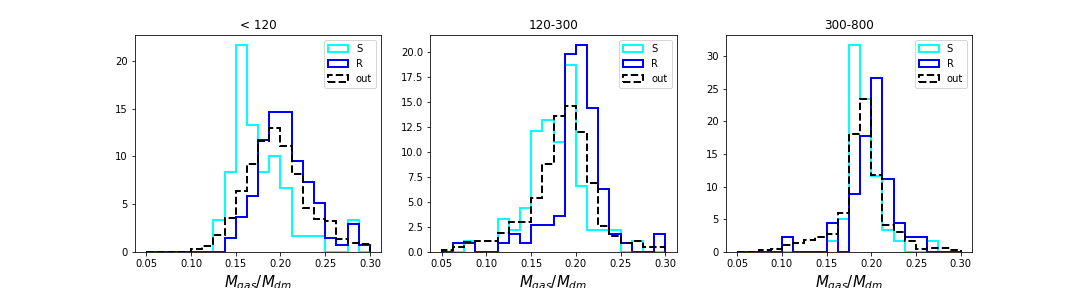
\includegraphics[width=10cm]{Figures/Fraccion_cortemasa.png}
\decoRule
\caption[asd]{Estas son las fracciones de masa de los halos, mirando el gas. Ahi puede haber algo con el void S, aunque son pocos halos :/}
\label{fig:Electron}
\end{figure}

\begin{figure}[h]
\centering
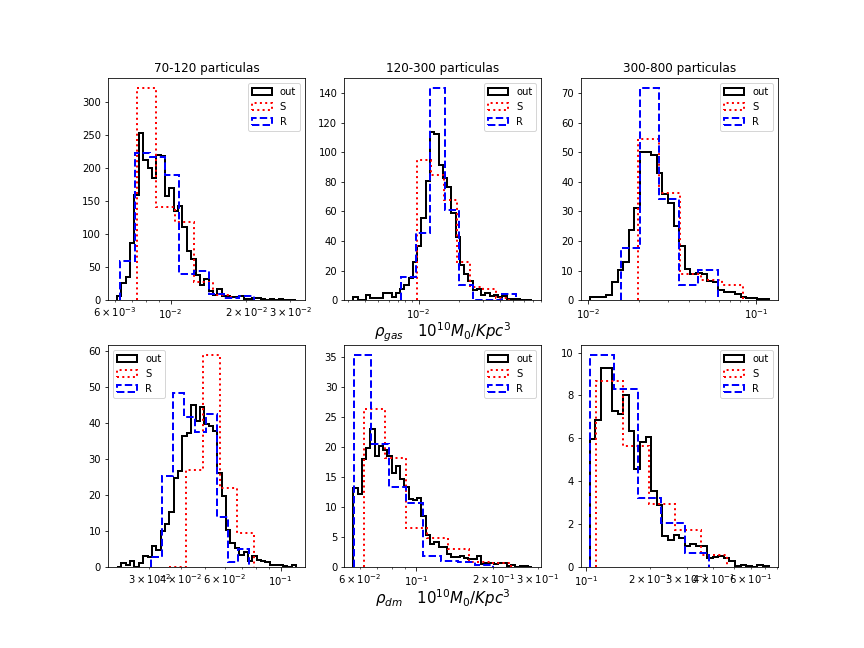
\includegraphics[width=10cm]{Figures/Densidades_cortemasa.png}
\decoRule
\caption[asd]{Estas son las densidades, estoy tomando particulas a dos radios viriales,entonces seria la masa de particulas dividido 2 radios viriales.  }
\label{fig:Electron}
\end{figure}

\begin{figure}[h]
\centering
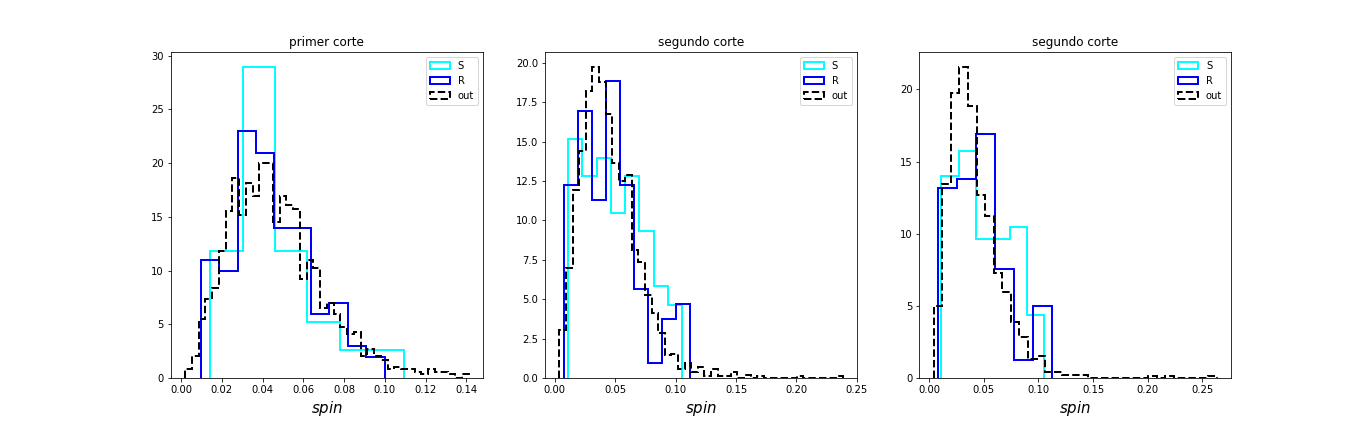
\includegraphics[width=10cm]{Figures/Spin_cortemasa.png}
\decoRule
\caption[asd]{Aca mire el spin de los halos, pero es solamente el spin que me tira rockstar  }
\label{fig:Electron}
\end{figure}

\begin{figure}[h]
\centering
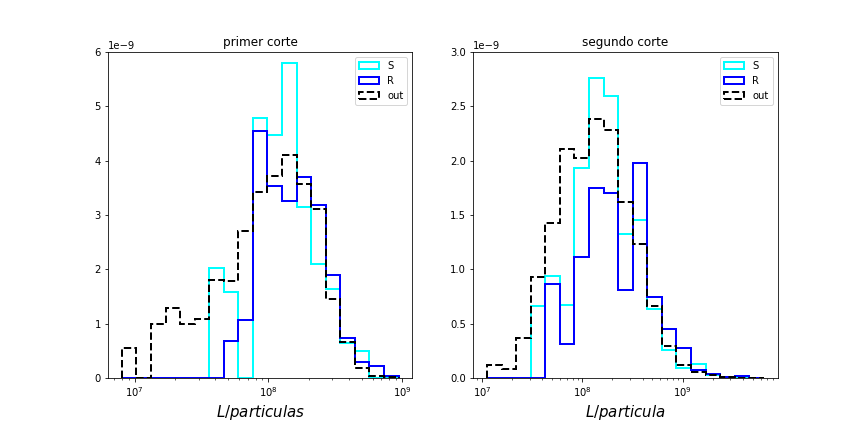
\includegraphics[width=10cm]{Figures/Momangular_cortemasa.png}
\decoRule
\caption[asd]{Aca tengo el modulo del momento angular (con las componentes que me tira rockstar) dividido el numero de particulas, donde estas particulas son tambien las que rockstar dice que tiene cada halo }
\label{fig:Electron}
\end{figure}

\begin{figure}[h]
\centering
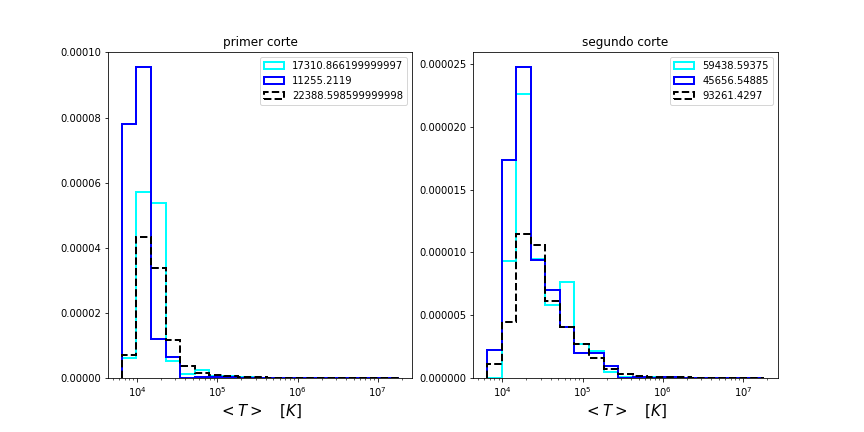
\includegraphics[width=10cm]{Figures/temperatura_cortemasa.png}
\decoRule
\caption[asd]{Y este tiene las temperaturas de los halos, el codigo de colores es el mismo que los plots anteriores y en el label lo que esta es la mediana de la temperatura, si pongo la promedio me da valores muy extremos, me queda a la izquierda : 4.7e4 K para los voids y 2.7e5 para fuera del void, derecha: 1.3e5 void S, 1.7e5 void R y 6e5 afuera}
\label{fig:Electron}
\end{figure}